\documentclass[a4paper,UTF8]{article}
%\usepackage{ctex}
\usepackage[margin=1.25in]{geometry}
\usepackage{color}
\usepackage{graphicx}
\usepackage{amssymb}
\usepackage{amsmath}
\usepackage{amsthm}
\usepackage{enumerate}
\usepackage{bm}
\usepackage{hyperref}
\usepackage{epsfig}
\usepackage{color}
\usepackage{mdframed}
\usepackage{lipsum}
\usepackage{mathtools}
\usepackage{algorithm}
\usepackage{algorithmic}
\newmdtheoremenv{thm-box}{myThm}
\newmdtheoremenv{prop-box}{Proposition}
\newmdtheoremenv{def-box}{define}

\setlength{\evensidemargin}{.25in}
\setlength{\textwidth}{6in}
\setlength{\topmargin}{-0.5in}
\setlength{\topmargin}{-0.5in}
% \setlength{\textheight}{9.5in}
%%%%%%%%%%%%%%%%%%set header and footer here%%%%%%%%%%%%%%%%%%
\usepackage{fancyhdr}                                
\usepackage{lastpage}                                           
\usepackage{layout}                                             
\footskip = 10pt 
\pagestyle{fancy}                    
\lhead{2024, Spring}                    
\chead{Computer Vision: Representation and Recognition}
\rhead{Assignment 3}                                                                                               
\cfoot{\thepage}                                                
\renewcommand{\headrulewidth}{1pt}  			%header
\setlength{\skip\footins}{0.5cm}    			
\renewcommand{\footrulewidth}{0pt}  		

\makeatletter 							
\def\headrule{{\if@fancyplain\let\headrulewidth\plainheadrulewidth\fi%
\hrule\@height 1.0pt \@width\headwidth\vskip1pt	
\hrule\@height 0.5pt\@width\headwidth  			
\vskip-2\headrulewidth\vskip-1pt}      			
 \vspace{6mm}}     						
\makeatother  

%%%%%%%%%%%%%%%%%%%%%%%%%%%%%%%%%%%%%%%%%%%%%%
\numberwithin{equation}{section}
\newtheorem{myThm}{myThm}
\newtheorem*{myDef}{Definition}
\newtheorem*{mySol}{Solution}
\newtheorem*{myProof}{Proof}
\newcommand{\indep}{\rotatebox[origin=c]{90}{$\models$}}
\newcommand*\diff{\mathop{}\!\mathrm{d}}

\usepackage{multirow}
\renewcommand\refname{reference}


\begin{document}
\title{Computer Vision: Representation and Recognition\\
Assignment 3}
\author{student ID, name, \href{mailto:your@email.address}{your@email.address}}
\maketitle

\section{Question 1}

\subsection{question1.1}
write down your answer here.

\subsection{question1.2}
if there are multiple steps, you can use enumerate as follows:

\begin{enumerate}[(\romannumeral1)]
	\item write your steps here,
	\item Latex supports powerful mathematical formulas, as following:

	\begin{equation}
		(I*F)[i,j]=\sum_{k,l}I[i-k,j-l]F[k,l].
	\end{equation}
	
	\item you can insert your result image:
	
	\begin{figure}[h]
		\centering  %centering image
		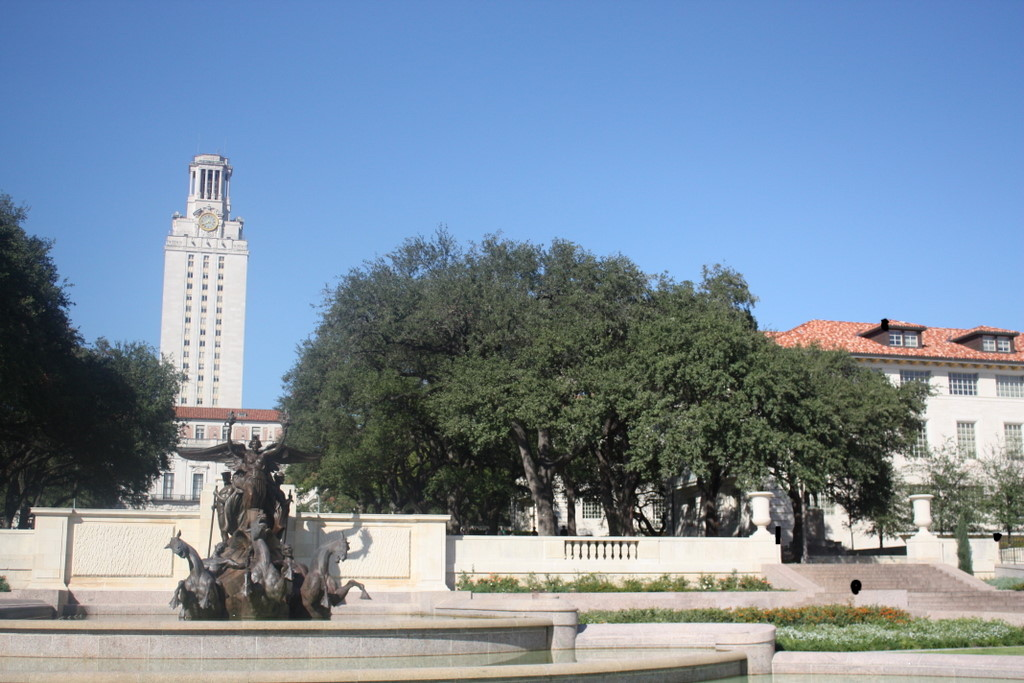
\includegraphics[width=5cm,height=5cm]{uttower2.jpg}  % load image
		\caption{this is a figure.}  %
		\label{fig:mcmthesis-logo}   %
	\end{figure}
	\item when you finish one question, write another section to start a new question.
	\item more powerful features waiting for you to discover.
	
\end{enumerate} 

\section{Question 2}

\subsection{question2.1}
write down your answer here.

\subsection{question2.2}

\bibliographystyle{plain}
\bibliography{ref}
\end{document}